\documentclass[a4paper,12pt]{article}

%\usepackage[pdftex]{graphicx}
\usepackage{amsmath}
%\usepackage[latin1]{inputenc}
%\usepackage{hyperref}
%\usepackage[T1]{fontenc}
%\usepackage[utf8]{inputenc}
%%GD Quand je mets usepackage[utf8]{inputenc} je n'arrive plus à compiler la biblio
%J'ai essayé de débuger : je n'y suis pas arrivé
\usepackage{rotating}
\usepackage{setspace}
\usepackage{lscape}
\usepackage[round]{natbib}
\usepackage{multirow}
\usepackage{rotating}
\usepackage{vmargin}
\usepackage{epstopdf}
\usepackage{hyperref}
\usepackage{float}
\usepackage{caption}
\usepackage[tableposition=top]{caption}
\usepackage{amsfonts}
\usepackage{bbold}
\usepackage{bbm}
\usepackage[flushleft]{threeparttable}
%\usepackage{bbold}
%\usepackage[T1]{fontenc}
% JH : impossible de compiler avec le package bbold, remplacé par amsfonts
% LP : impossible de compiler avec le package bbold, remplacé par bbm
\usepackage{upgreek}
\usepackage{comment}
\includecomment{commentGD}
\usepackage[draft]{todonotes}
%\usepackage[disable]{todonotes}
%%GDPour cacher les notes, \usepackage[disable]{todonotes}

\usepackage{setspace}

%\usepackage[nolists, figuresfirst]{endfloat}
%\usepackage{sidefloat}

\setlength{\abovecaptionskip}{-8pt}

%\usepackage[usenames]{color}
%\definecolor{grey}{rgb}{0.35,0.35,0.35}
%\definecolor{webdarkblue}{rgb}{0,0,0.4}
%\definecolor{orange}{rgb}{0.7,0.2,0.05}


%\usepackage[pdfcreator={PDFLaTeX}, pdfproducer={PDFLaTeX}, pdfstartview=FitH, pdfpagemode=UseOutlines, pagebackref=false, colorlinks={true},
%citecolor={webdarkblue}, linkcolor={webdarkblue},
%urlcolor={webdarkblue}]{hyperref}



%\addtolength{\oddsidemargin}{-0.4in}
%\addtolength{\evensidemargin}{-0.4in}
%\addtolength{\textwidth}{0.8in} \addtolength{\topmargin}{-0.85in}
%\addtolength{\textheight}{1.7in}
\renewcommand{\baselinestretch}{1.2}

\newcommand\cites[1]{\citeauthor{#1}'s\ (\citeyear{#1})}

\newcommand\citeh[1]{\citeauthor{#1}'\ (\citeyear{#1})}

\setmarginsrb{3cm}{2cm}{3cm}{2cm}{0,5cm}{0,5cm}{0,3cm}{0,5cm}



% commands

\newcommand{\bi}{\begin{itemize}}
\newcommand{\ei}{\end{itemize}}
\newcommand{\be}{\begin{enumerate}}
\newcommand{\ee}{\end{enumerate}}
\newcommand{\bd}{\begin{description}}
\newcommand{\ed}{\end{description}}
\newcommand{\beqa}{\begin{eqnarray}}
\newcommand{\eeqa}{\end{eqnarray}}
\newcommand{\beq}{\begin{equation}}
\newcommand{\eeq}{\end{equation}}
\newcommand{\bs}{\bigskip}
\newcommand{\A}{$^a$}
\newcommand{\B}{$^b$}
\newcommand{\C}{$^c$}

\renewcommand{\baselinestretch}{1.2}
%\doublespacing

%\linespread{1.6}

%\newcommand{\note}[1]{\footnote{\begin{doublespace}#1\end{doublespace}}}


\begin{document}


\title{\textsc{International Transport costs:\\New Findings from modeling additive costs} \\
Asnwer to Referee 1}

\author{Guillaume \textsc{Daudin}\thanks{%
University Paris-Dauphine \& PSL University, IRD, LEDa, UMR 225, DIAL, 75016 Paris, France; email: \url{guillaume.daudin@dauphine.psl.eu}}  \qquad J\'{e}r\^{o}me \textsc{H\'{e}ricourt} \thanks{Universit\'{e} de Lille - LEM-CNRS UMR 9221, France \& CEPII, France; email: \url{jerome.hericourt@univ-lille.fr}}\qquad Lise \textsc{Patureau}\thanks{Corresponding author.
University Paris-Dauphine \& PSL University, LEDa, 75016 Paris, France;  email: \url{lise.patureau@dauphine.psl.eu} } }


\date{July 2020}
 \maketitle
\bigskip

\section{Critique 1: Empirical Strategy}

\subsection{Deriving the share of additive costs in total transport costs \label{ssec:interpret_beta}}
With $i$ the origin country, $k$ the product category at the HS6 level (and reasoning at the year- transport mode level), $p_{ik}$ the import (cif) price and $\tilde{p}_{ik}$ the export (fas) price, transport costs $f_{ik}\equiv \frac{p_{ik}- \tilde{p}_{ik}}{\tilde{p}_{ik}} $ are written in Hummel's terminology as:


\begin{equation}
f_{ik} = X_{is(k)}\tilde{p}_{ik}^{-\beta_{ik}} \label{eq:Hummels}
\end{equation}

It is trivial to show that:
$$\frac{\partial f_{ik}}{\partial \tilde{p}_{ik}} \frac{\tilde{p}_{ik}}{f_{ik}}= -\beta_{ik}$$

Then
\begin{itemize}
\item If $\beta_{ik} = 0$, then $p_{ik} = (1+X_{is(k)})\tilde{p}_{ik}$: Only ad-valorem transport costs
\item If $\beta_{ik} = 1$, then $p_{ik}=\tilde{p}_{ik}+X_{is(k)}$: Only additive costs
\end{itemize}

This suggests that, the closer $\beta_{ik}$ to 1, the more prevalent additive costs in total transport costs. Can $\beta_{ik}$ be related to the share of additive costs in total transport costs? The answer is positive. To show this clearly, start from:

\begin{eqnarray*}
f_{ik} &=& \frac{p_{ik}-\tilde{p_{ik}}}{\tilde{p}_{ik}}\\
\text{with}:&& p_{ik} = \tau_{is(k)}\tilde{p}_{ik} + t_{is(k)} \\
\end{eqnarray*}

assuming that transport costs decompose in two components, additive transport costs $t_{is(k)}$ and multiplicative costs (ad-valorem) $\tau_{is(k)}$, supposed to be identical in the product-dimension for any $k$ product within the 3-digit classification $s$ it belongs to.

This gives:

$$f_{ik} = \frac{(\tau_{is(k)}-1)\tilde{p}_{ik}+t_{is(k)}}{\tilde{p}_{ik}}$$

From this, we have

\begin{eqnarray*}
\frac{\partial f_{ik}}{\partial \tilde{p}_{ik}} &=& \frac{(\tau_{is(k)}-1)\tilde{p}_{ik} - ((\tau_{is(k)}-1)\tilde{p}_{ik} +t_{is(k)})}{\tilde{p}_{ik}^2} \\
&=& \frac{-t_{is(k)}}{\tilde{p}_{ik}^2}
\end{eqnarray*}

Hence
\begin{eqnarray*}
\frac{\partial f_{ik}}{\partial \tilde{p}_{ik}} \frac{\tilde{p}_{ik}}{f_{ik}}&=& \frac{-t_{is(k)}}{(\tau_{is(k)}-1)\tilde{p}_{ik} +t_{is(k)}}\\
&=& \frac{-\frac{t_{is(k)}}{\tilde{p}_{ik}}}{\tau_{is(k)}-1 +\frac{t_{ik}}{\tilde{p}_{ik}}}
\end{eqnarray*}

This shows that $\beta_{ik}$ can be interpreted as the share of additive costs in total transport costs:

$$\beta_{ik} = \frac{\frac{t_{is(k)}}{\tilde{p}_{ik}}}{\tau_{is(k)}-1 + \frac{t_{is(k)}}{\tilde{p}_{is(k)}}} $$

\subsection{Coming back to the Referee's 1 concern}

In italics, I report the Referee's comment. Into brackets in bold characters inserted into the referee's statement, my comment.

\textit{Using the notation of the authors, they are intreated
in identifying the share of the specific cost in the total transport cost.} \textbf{\[In fact, he/she forgets that with our identification strategy, we do not only identify the share of additive costs, but also their level. This might be a route to follow for the ``big picture part''\]}.


\textit{ Namely,}
\begin{eqnarray*}
&& \frac{\frac{t_{is(k)}}{\tilde{p}_{ik}}}{\tau_{is(k)}-1 + \frac{t_{is(k)}}{\tilde{p}_{is(k)}}} \\
\text{or,} &&\frac{t_{is(k)}}{(\tau_{is(k)}-1)\tilde{p}_{is(k)} + t_{is(k)}}
\end{eqnarray*}

\textit{The way they approach the problem is that they assume that (a) $\tau_{ik} = \tau_i\tau_{k}$,
(b) $t_{ik} = t_i +t_k$, and (c) $t_k$ and $\tau_k$ are uniform across products within industry
s. After imposing these assumptions, they estimate the following specification}

\begin{equation}
\ln\left(\frac{p_{ik}}{\widetilde{p}_{ik}}-1 \right)= \ln \left(\tau_{i} \times \tau_{k}+\frac{t_{i} + t_{k}}{\widetilde{p}_{ik}}-1 \right) + \epsilon_{ik} \label{eq:equation0}
\end{equation}

\textit{in which $\tau_i$, $\tau_{s(k)}$, $t_i$, and $t_{s(k)}$ are identified as fixed effects coefficients.
In my opinion this choice of strategy is quite sub-optimal, as (i) it relies on
the strong assumptions highlighted above, (ii) it is computationally expensive
as noted by the authors on multiple occasions, and (iii) it is subject to an
endogeneity problem, which the authors disregard with one sentence, but which
is rather detrimental in my opinion.}

The three points raised by the referee are all equally important, and we answer separately to each of them below.



\paragraph{(i) On the assumptions underlining our empirical approach}
Our main empirical equation and its underlying assumptions regarding the separability of transport costs between their country- and product-level components draw on the one proposed by Irarrazabal, Moxnes and Opromolla (the Review of Economics and Statistics, 2015) to estimate the share of additive costs in a firm-level context. It relies on a simple theoretical framework with minimal assumptions, and is compatible with most approaches within the so-called category of ``New Trade Theories''. More importantly, this formulation allows us recovering explicitly the \textbf{levels of}, respectively, additive and multiplicative costs. Despite its formal elegance and simplicity, this is not possible in such a straightforward manner with the Hummels' methodology, which only recovers the \textbf{share} of additive in total transport costs. \textbf{elaborate on this in the Big Picture part.}

Nevertheless, to take full account of the referee’s remark, we decided run an additional set of estimations based on the Hummel's methodogy as proposed by the referee, based on Equation (\ref{eq:estimation_ref1}). This is developed in Section XX of this letter.

\textbf{We need to explain why not in the main text, but in the (online?) appendix}

\paragraph{(ii) On the use of non-linear least squares (NLS)}
As highlighted by the referee, our estimated equation imposes to use non-linear estimation methods, such as Non-Linear Least Squares. However, even with another formulation, such as the one suggested by the referee in Equation (\ref{eq:estimation_ref1}), we would still be constrained to resort to non-linear estimators. This is due to the restrictions imposed \textit{ex-ante} on parameters, i.e. $\tau \geq 1$ and $t geq 0$, the latter meaning simply we constrain both types of trade costs to be non-negative. Without these restrictions, standard linear, least squares estimates often deliver aberrant values with more than mild quality-of-fit [insert examples here]
We do acknowledge this is very important point was not made clear enough in the initial version, and did our best to make the pint clear in the revised version [see page XX : XX insert quote XX].

\paragraph{(iii) Endogeneity problem}
Indeed, this is a very important point. The referee states that, based on theoretical insights by Melitz (Econometrica, 2003) or Baldwin and Harrigan (AER, 2011), $1/\tilde{p}_{ik}$ is correlated in one direction on another with residuals $\epsilon_{ik}$. In other words, more productive firms and/or firms selling high-quality products will charge higher prices, all other things equal – in our case, for a given country-product pair.
We obviously do not question this conceptual issue. However, it is worth noting that a good deal of the bias (actually, the part relating to the quality effect) is going to appear identically in the CIF ($p$) and the FAS ($\tilde{p}$) prices. Consequently, since our dependent variable is based on a ratio between the former and the latter, the (reverse causality) bias cancels out. That said, remains the possibility that bigger firms may impact transport costs, due to their ability of bargaining discounts for larger shipped volumes.


Following the referee's advice, we decided therefore to provide some IV-estimates to provide a clean assessment of the size of the potential bias.


XXX At some point, explain HS10 duty do not exist, contrary to what the referee asserts. At best, it was HS6 or HS8 XXX


\subsection{Exploring Referee's alternative functional form}


\textit{A more natural approach is what the authors, at some point, refer to as the
Hummel's Methodology. That is, one can alternatively estimate the share of the
additive component as:}

$$\frac{t_{ik}}{ (\tau_{ik}-1)\tilde{p}_{ik} + t_{ik}} = \beta_{ik}$$

\textit{where $\beta_{ik}$ is the elasticity of transport costs w.r.t. unit price} [\textbf{in absolute value, see Equation \ref{eq:Hummels}}]. \textit{Given the authors' objective and the data they are using, $\beta$ can be separately estimated
for each industry-country pair using the following regression:}

\begin{equation}
\ln f_{ikd} = \beta_{is(k)}\ln \tilde{p}_{ikd} + \text{Controls}_{ikd} +\epsilon_{ikd} \label{eq:estimation_ref1}
\end{equation}

\textit{where $d$ denotes the US district of entry and $k$ denotes an HS10 product. The
identification of $\beta_{ik}$, in this case, would rely on the across HS10 product and
district-of-entry variation in $f_{ik}$ and $p_{ik}$. Estimating the above equation would
obviously require that the authors do not aggregate up the raw Census data
across all districts and all 10-digit products pertaining to the same 5-digit category.}

\textit{The first advantage of this so-called Hummel's Approach is that the above
regression can be estimated separately for various country-industry pairs, without
imposing Assumptions (a) and (b), outlined above.}

\textbf{I report here the referee's footnote: Should we deal with this? If he/she is not convinced because small sub-sample, do it on a much larger sample? This would better convince him that the separability assumption is not an issue.}: \textit{The authors do check the robustness of their results w.r.t. the separability assumption, but this only done for a small sub-sample.}



\textbf{There is also a point here, about the degree of sectoral classification. In our paper, $k$ = 5 digit and $s(k)$ = 3 digit. He/she suggests that, in the estimated equation, $k$ = 10 digit and $s(k)$= 5 digit. Which means, having an estimated $\beta$ specific to the origin country-5-digit level. I need to have a refresher on this: What have we done finally? and why?}


XXX Say something about the fact that in the original US-custom data, the finest degree of sectoral classification is 8-digit, not 10? XXX

\subsubsection{What we do}

Our estimated equation is written as:
\begin{equation}
\ln\left(\frac{p_{ik}}{\widetilde{p}_{ik}}-1 \right)= \ln \left(\tau_{i} \times \tau_{k}+\frac{t_{i} + t_{k}}{\widetilde{p}_{ik}}-1 \right) + \epsilon_{ik} \label{eq:equation0}
\end{equation}

\noindent with $s$= 3 (or 4) digit and $k$=5 digit (based on Hummel's original dataset from 1974-2004). We thus exploit the variability of transport costs between countries and between 3-digit sectors (conditional on a year and a transport mode, air or vessel). To sum up our methodoly:
\begin{itemize}
\item Estimating Equation \ref{eq:equation0} provides us with estimates of $\hat{t}_i$, $\hat{t}_{s(k)}$, $\hat{\tau}_i$, $\hat{\tau}_{s(k)}$.
\item We rebuild
\begin{eqnarray*}
\hat{t}_{is(k)} &= &\hat{t}_{i}+\hat{t}_{s(k)} \\
\hat{\tau}_{is(k)} &= & \hat{\tau}_{i}\times\hat{\tau}_{s(k)}
\end{eqnarray*}
\item We deduce the weighted average value of each component $\bar{t}$, $\bar{\tau}$ by year and transport mode, the weighting scheme being the relative value of the flows for each $i,s$ flow, as well as the median, the maximum and the minimum values.
\item With this in hand, we can (among other things) obtain the estimated share of additive costs in total transport costs for each $i,k$ flow:


$$\hat{\beta}_{ik} = \frac{\frac{\hat{t}_{is(k)}}{\tilde{p}_{ik}}}{\tau_{is(k)}-1 + \frac{t_{is(k)}}{\tilde{p}_{is(k)}}} $$
\end{itemize}

\subsubsection{What the referee suggests to do}

The estimation strategy suggested by the referee starts from Equation (\ref{eq:Hummels}) linking transport costs and unit prices as assumed in Hummels (2007). As shown in Subsection (\ref{ssec:interpret_beta}), the elasticity of transport costs to unit prices $\beta_{ik}$ in Equation (\ref{eq:Hummels}), also corresponds to the share of additive costs in total transport costs. The share of aditive costs can hence be encovered by regressing transport costs on unit (ie, fas) prices. Specifically, the referee suggests to run the estimation based on Equation (\ref{eq:estimation_ref1}).

Precisely, by year and transport mode, this implies running the estimation for each country of origin $i$ and each sector $s(k)$ = 3 digit sector (\textbf{why 3-digit? and not 5 as suggested by the referee?}, exploiting the variability between sub-sectors at the 8 digit level ($k$) and between ports of entry in the US ($d$).

\subsubsection{Strategy of answer}

\paragraph{a) The advantages are not as important as suggested by the referee}
\begin{itemize}
\item[Advantage 1]: One is not compelled to assume separability between the country-component and the product-component of transport costs.
\item[$\Rightarrow$] Answer can be in 2 parts: 1) This is not a strong assumption - better convince him/her: Run the robustness to the separability assumption on a larger sample; 2) Show that the estimated $\beta$ is not that different between the two methods.
\item[Advantage 2]: There is a handful of instruments (HS-8 product-specific tariff rates or lagged prices) to instrument fas prices
\item[$\Rightarrow$] Answer: When we instrument fas prices at the 5-digit level using tax duties (still using our own methodology), we do not obtain much different results. \textbf{But he/she suggests to do it on HS-8 fas prices, not 5-digit prices, and to imply his estimated equation. Have we done that?}
\item[Advantage 3]: A more transparent comparison with Hummel (2007): How to answer to this point? Re-read the paper to see if we are clear enough?
\end{itemize}

\paragraph{b) The costs are high}
\begin{itemize}
\item[Concern 1] The suggested estimation strategy implies having much less data to exploit, for two reasons.
\begin{enumerate}
\item Information about the port of entry are only available in the recent years (\textbf{since when? why? before, we rely on Hummel's data set, but we could buy the original US custom data for 1974-2004? Or even in those dataset it does not exist?}). In our view, the historical coverage is interesting per se, as it provides useful insights about how transport costs have evolved over time, and most importantly how the specific values of the additive and ad-valorem transport costs components have evolved over time. Eliminating this dimension of the paper would be detrimental to its value-added.
\item As underlined before, the method is run country by country, and 3-digit sector by 3-digit sector, exploiting the variability within each country-3d sector across 8-d sub-sectors and ports of entry. Yet, it appears that for many couples (country, 3-digit sector), there is too few variability across sub-sectors (even at the HS-6 digit classification) or ports en entry given the number of fixed effects included in the regression, such that estimation can not be run. This can be seen comparing the number of observations by year/ transport mode with our method / with the referee's method reported in Table XXX \textbf{TO DO}. Put it differently, this methodology discards countries which export a limited range of goods to the US and/or which arrive in the USA through the same ports of entry. In this respect, the induced selection bias reduces the general scope of our transport costs estimates. For things to be comparable across methods, we have thus re-run our estimation strategy on the same sample of observations as the one used in the referee's method.

    \end{enumerate}
\item[Concern 2] The suggested estimation method implicitly assumes that transport costs of say, tissues, have nothing in common whether those goods comes from France or from Bangladesh; or that transport costs that apply to imported goods from France have no common component across sectors; in both cases, one might view this as a disputable assumption. By contrast, we suppose that transport costs are sector-country specific. \textbf{FAIRE REFERENCE A DES PAPIERS EN TRADE QUI ONT DES TRADE COSTS Pays-spécifique?}
\item[Concern 3] The suggested estimation method does not allow to recover the values of each component of transport costs separately, but only the relative shares; while our methodology drives an estimate for each component ($\tau$, $t$) from which we can deduce the relative share of each. In this respect, we gain in generality. \textbf{DEEPEN this for the Big picture part}.
\item[Concern 4] The suggested method features less accuracy in the estimation of the $\beta$. Considering the value of the $\beta$ by itself, there is no criteria to discriminate between the value estimated with our method and the one obtained with the suggested method (when, of course, run on the same sample). Things are more clear-cut in terms of accuracy of the estimation. Specifically, our method yields a more precise estimation of the $\beta$ than the referee's method. To develop on this, for each year and transport mode:
    \begin{itemize}
    \item With the referee's method, we estimate one value for the share of additive component $beta$ at the $i,s$ level denoted $\hat{\beta}^{ref}_{is(k)}$ associated with a standard deviation $SD_{is}$. From this, we can deduce the 5- 95\% threshold values through:
        $$\hat{\beta}_{is}^{min,ref} = \hat{\beta}^{ref}_{is(k)} - 1.96 SD_{is},\quad \hat{\beta}_{is}^{max,ref} = \hat{\beta}^{ref}_{is(k)} + 1.96 SD_{is}$$
     
    \item  With our method, one estimation allows to calculate each transport cost component $\hat{t}_{is}$, $\hat{\tau}_{is}$ and an associated $\beta_{is}$. We generate a distribution of $\beta$ through bootstrap method (10,000 random draws), from which we can compute the mean, the median and the 5-95 threshold values for each couple $i,s$.
    \item We can then evaluate the accuracy of each estimation method by comparing the distributions of the $\beta$. This is reported in the Figures XXX (for Air) and XXX (for Vessel). Our method undoubtedly yields more accurate estimations of the share of additive components, whatever the transport mode considered. For sake of brevity, we report the mean distribution averaged over the period, a similar conclusion applies on a yearly basis. \textbf{Averaged over the two transport modes? For only one?}
        

\begin{figure}[htbp]
\caption{Accuracy of the estimation of the $\beta$: Comparison}
\label{fig:accuracy_beta}
\begin{center}
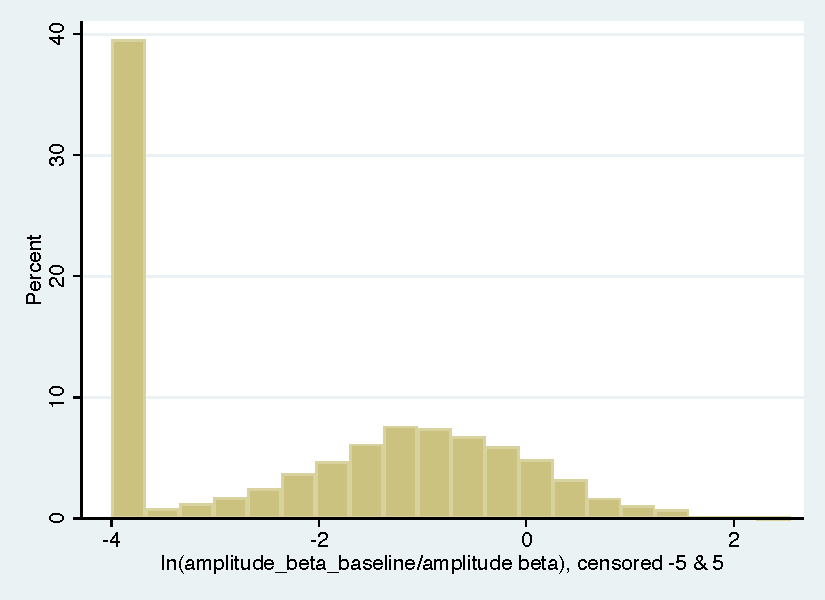
\includegraphics[height=4in]{accuracy_beta.pdf}
\end{center}
\end{figure}

Figure \ref{fig:accuracy_beta} reports the log of the interval confidence of the $\beta$ obtained with our methodology (with bootstrap), relative to the one obtained with the referee's method. \textbf{average over the years? the transport modes? unclear}. In most cases, the log of the ratio is negative, implying a lower interval confidence of the $\beta$ estimate with our methodology.
        
    \end{itemize}
\end{itemize}


\textbf{Where are the results comparing the estimates of the $\beta$, in value? I don't find these results anymore...}

\end{document} 